\documentclass[conference]{IEEEtran}
\IEEEoverridecommandlockouts
\usepackage{cite}
\usepackage{amsmath,amssymb,amsfonts}
\usepackage{algorithmic}
\usepackage{graphicx}
\usepackage{textcomp}
\usepackage{xcolor}
\usepackage{booktabs}
\usepackage{url}
\usepackage{float}
\usepackage{hyperref}
\def\BibTeX{{\rm B\kern-.05em{\sc i\kern-.025em b}\kern-.08em
    T\kern-.1667em\lower.7ex\hbox{E}\kern-.125emX}}
\begin{document}

\title{GPU Accelerated GGM PRF Tree Construction:\\
AES-128 vs.\ BLAKE2s Performance--Security Analysis}

\author{
\IEEEauthorblockN{Kevin Liang \quad Bryce Blair \quad Ryan Luo}
\IEEEauthorblockA{
\textit{Dept. of Electrical and Computer Engineering} \\
\textit{University of California, San Diego} \\
La Jolla, CA, USA}
}

\maketitle

\begin{abstract}
We implement the Goldreich Goldwasser Micali (GGM) pseudorandom function (PRF) tree construction entirely from scratch on the GPU, using two different length doubling pseudorandom generators (PRGs): AES-128 and BLAKE2s. Both primitives are written from scratch on both CPU and GPU, with no reliance on cryptographic libraries. The CPU reference paths (pure-Python AES-128, an independent pure-C AES, and a from-scratch pure-Python BLAKE2s) are validated against NIST FIPS 197 known-answer vectors, and a BLAKE2s reference, and the GPU kernels (CuPy RawKernel, CUDA C) are verified byte-exact against the CPU outputs at tree depths 4, 8, and 12 for both PRGs. On an NVIDIA GPU, we benchmark full tree expansion across depths 4 through 16 (16 to 65,536 leaves). The GPU reaches 38.1 million leaves/s for AES and 82.4 million leaves/s for BLAKE2s, with measured GPU/CPU speedups up to 8,298$\times$ for AES and 45,975$\times$ for BLAKE2s. Because both CPU baselines are written from scratch, the comparison is fair, and BLAKE2s is the faster primitive on both axes: it achieves the highest absolute GPU throughput and the largest speedup over its CPU baseline, consistent with its add-rotate-xor design mapping more efficiently onto GPU integer units than AES's table lookup and finite-field rounds.
\end{abstract}

\begin{IEEEkeywords}
GGM construction, pseudorandom function, pseudorandom generator, GPU, CUDA, CuPy, AES, BLAKE2s, parallel cryptography
\end{IEEEkeywords}

\section{Introduction}

\paragraph{Motivation}
The Goldreich Goldwasser Micali (GGM) construction~\cite{ggm1986} is a foundational result in theoretical cryptography. It shows that a secure pseudorandom function (PRF) can be built from any length-doubling pseudorandom generator (PRG). Starting from a single secret seed, the construction defines a complete binary tree in which each node is expanded by the PRG into its two children, and the $2^d$ leaves at depth $d$ are the PRF outputs indexed by their $d$-bit path from the root. The GGM tree underlies a wide range of modern primitives, including puncturable PRFs, distributed point functions, and the seed expansion phase of function secret sharing, where very large trees must be expanded quickly. This makes the efficiency of tree expansion a practical concern rather than just a theoretical issue.

\paragraph{Why GPU}
The GGM tree is a logical target for GPU acceleration because expansion is parallel within each level. Every node at level $\ell$ depends only on its own parent seed, so all $2^\ell$ nodes at a level can be expanded simultaneously and independently. A GPU can therefore process an entire level in a single kernel launch with one thread per node, and the tree is built level by level until the desired depth is reached. The question then becomes not whether the GPU can help but by how much, and how that answer depends on the choice of PRG.

\paragraph{Obstacles}
Implementing the construction from scratch can present several difficulties. The two PRGs must be byte-to-byte correct since a single bit error in a round function silently produces a wrong but plausible-looking output. AES-128 requires a correct S-box, key schedule, and finite-field \texttt{MixColumns} step in $\mathrm{GF}(2^8)$, while keyed BLAKE2s requires faithful reproduction of the RFC 7693 parameter block, message schedule, and finalization flags. The GPU implementations must then match the CPU implementations exactly despite differences in memory layout, endianness handling, and the absence of standard headers in the CuPy NVRTC compilation environment. Finally, meaningful benchmarking requires careful treatment of GPU timing so that measurements capture true kernel completion rather than asynchronous launch enqueue time.

\paragraph{Our approach}
We build a modular pipeline with a clean separation between the PRG and the tree expansion logic. A single \texttt{GGMTree} class parameterized by PRF, device, and depth drives expansion. Each PRG provides a CPU-level expansion function and a GPU-level expansion function with identical semantics. Both PRGs are implemented from scratch on both devices: AES-128 in pure Python and in CUDA C, as well as keyed BLAKE2s in pure Python (CPU) and in CUDA C (GPU). A dedicated test establishes correctness against published standards and checks the GPU against the CPU, and a separate benchmark harness measures throughput and speedup across tree depths.

\paragraph{Contributions}
\begin{itemize}
\item From-scratch implementations of two length-doubling PRGs (AES-128 and BLAKE2s) on both CPU and GPU, with AES additionally implemented independently in pure C as a third reference.
\item A GPU GGM tree expander (CuPy RawKernel, CUDA C) that keeps all data on the device between levels and transfers only the final leaf array back to the host.
\item Correctness validation tests validating CPU paths against NIST FIPS 197 vectors and a BLAKE2s reference, and verifying GPU/CPU byte exact agreement for both PRGs at depths 4, 8, and 12.
\item A benchmark across depths 4-16 reaching 82.4~million leaves/s (BLAKE2s, GPU) and speedups up to $45{,}975\times$ (BLAKE2s) over a from-scratch CPU baseline.
\item A performance \& security analysis comparing the two PRGs on a fair footing, with both CPU baselines implemented from scratch.
\end{itemize}

\section{Background and Related Work}

\paragraph{The GGM construction}
The GGM construction~\cite{ggm1986} converts a length-doubling PRG $G:\{0,1\}^n \to \{0,1\}^{2n}$ into a PRF. Writing $G(k) = (G_0(k), G_1(k))$ for the left and right halves of the output, the PRF keyed by seed $s$ is defined on a $d$-bit input $x = x_1 x_2 \cdots x_d$ by the iterated composition $F_s(x) = G_{x_d}(\cdots G_{x_2}(G_{x_1}(s))\cdots)$. Evaluating the function at every input simultaneously is exactly a breadth-first expansion of a complete binary tree of depth $d$, which is the workload we accelerate. The security of the construction is reductive, so if $G$ is a secure PRG, then $F$ is a secure PRF, so the security of the whole tree rests entirely on the security of the chosen PRG.

\paragraph{PRG instantiations}
We instantiate the PRG in two ways. For AES-128 we define $G(k) = \mathrm{AES}_k(0^{128}) \,\|\, \mathrm{AES}_k(1\|0^{120})$ encrypting two fixed and distinct plaintexts under the node key $k$ in ECB mode. For BLAKE2s we define $G(k) = \mathrm{BLAKE2s}(\text{key}{=}k, \texttt{0x00}) \,\|\, \mathrm{BLAKE2s}(\text{key}{=}k, \texttt{0x01})$ with 16 byte digests. In both cases, the two halves are produced by applying the keyed primitive to two fixed, distinct inputs, which yields the two independent child seeds required by the construction. ECB mode is sound in this specific setting because each node key is used exactly once, and the plaintexts are fixed and public. Thus there is no chaining relationship between sibling nodes to leak, so no IV is required.

\paragraph{AES and BLAKE2s}
AES-128~\cite{fips197} is a 10-round substitution permutation block cipher and is the most widely deployed block cipher in practice. As a pseudorandom permutation, it is a natural and conservative PRG choice. BLAKE2s~\cite{rfc7693} is a fast cryptographic hash derived from the ChaCha permutation, designed explicitly for speed in software while retaining a strong security margin. In keyed mode, it functions directly as a PRF. The two represent a meaningful design contrast where a hardware-oriented block cipher whose per-call cost is dominated by table lookups and finite-field arithmetic, compared to a software-oriented ARX hash built from add-rotate-xor operations that map efficiently onto general-purpose registers.

\paragraph{GPU cryptography}
Prior work on GPU cryptography has repeatedly demonstrated that symmetric primitives map well onto data-parallel hardware when many independent blocks are processed at once. Our contribution is not a novel cipher implementation but a focused, controlled comparison of two PRGs inside an identical GGM tree harness, holding the parallelization strategy, memory layout, and measurement methodology fixed so that the only variable is the PRG itself.

\section{Method and Approach}
\label{sec:method}

\subsection{System Overview}
The system is organized around a single driver class, \texttt{GGMTree}, parameterized by the PRF (\texttt{aes} or \texttt{blake2s}), the device (\texttt{cpu} or \texttt{gpu}), and the tree depth. Expansion proceeds breadth-first: the root seed forms level 0, and each level is produced from the previous one by a level-expansion function that maps $N$ parent seeds to $2N$ child seeds. The driver is agnostic to the PRG and the device, as it simply calls the appropriate level expansion function $d$ times. This separation lets the same tree logic exercise four distinct backends (two PRGs $\times$ two devices) and guarantees that the CPU and GPU paths expand the tree identically at the structural level.

\subsection{Memory Layout}
At every level, the set of node seeds is stored as a contiguous \texttt{(N, 16)} array of unsigned bytes in row major order, so that each node's 16 bytes are stored contiguously. On the GPU, this layout is deliberate as adjacent threads process adjacent nodes. Because each node's bytes are contiguous, adjacent threads read adjacent regions of global memory. This produces coalesced memory access within a warp (32 threads) where the hardware can service the reads of many threads with a small number of wide memory transactions rather than many scattered ones. The same layout is used on the CPU so that the two paths are directly comparable and so that the host/device transfer is a single flat copy.

\subsection{Parallelization Strategy}
Each GPU kernel launch expands exactly one level of the tree. A thread is assigned to each parent node via the standard \texttt{blockIdx.x * blockDim.x + threadIdx.x} index, with 256 threads per block and enough blocks to cover all $N$ parents. The thread reads its 16-byte parent key, evaluates the PRG, and writes the two 16-byte children to their positions in the output array. No explicit inter-level synchronization barrier is required since each level is a separate kernel launch in the default CUDA stream, and CUDA guarantees that operations within a stream execute in order, so level $\ell$ is fully complete before level $\ell{+}1$ begins. Critically, the seed data remains resident on the GPU across all levels, so the final leaf array is copied back to the host. This keeps the PCIe bus idle during computation and avoids the classic mistake of shuttling intermediate results back and forth between host and device.

\subsection{AES-128 PRG}
The AES-128 PRG is implemented three times. The pure-Python CPU version implements the full cipher (key schedule with \texttt{RotWord}/\texttt{SubWord}/\texttt{Rcon}, \texttt{SubBytes}, \texttt{ShiftRows}, \texttt{MixColumns} via the \texttt{xtime} $\mathrm{GF}(2^8)$ doubling primitive, and \texttt{AddRoundKey}) and serves as the readable reference. An independent pure C implementation computes the same cipher using log/antilog tables for finite field multiplication, providing a second, structurally different reference that guards against a shared implementation bug. The GPU version is a CuPy RawKernel in CUDA C where each thread expands the 11 round key schedule into a 176 byte buffer, places the AES S-box and round constants in \texttt{\_\_constant\_\_} memory to avoid repeated global memory lookups, and encrypts the two fixed plaintexts to produce both children.

\subsection{BLAKE2s PRG}
The BLAKE2s PRG is implemented from scratch on both devices. The CPU version is written in pure Python following RFC 7693, where it implements the \texttt{G} mixing function, the ten-round compression with the \texttt{SIGMA} message permutation schedule, the keyed parameter block, and the two block keyed hash, with all 32-bit arithmetic explicitly masked to emulate word overflow. The GPU version is a CuPy RawKernel that mirrors the same logic in CUDA C, with the initialization vector and \texttt{SIGMA} table held in \texttt{\_\_constant\_\_} memory so that each thread's working state stays in registers. The keyed first block is the 16-byte key padded to 64 bytes with the byte counter set to 64, and the data block is a single byte padded to 64 with the counter at 65 and the finalization flag set. A practical obstacle arose here where the CuPy NVRTC compilation environment on the target machine could not locate the standard \texttt{<stdint.h>} header, so the fixed-width integer types were defined directly in the kernel source, mirroring the header-free style already used by the AES kernel.

\subsection{Correctness Methodology}
Correctness is established in several layers. The AES CPU implementation is checked against two NIST FIPS 197 known answer vectors, and the pure C implementation is independently confirmed to produce identical ciphertext. The BLAKE2s CPU implementation is checked against a reference BLAKE2s for random keys. Level expansion is checked for self-consistency by confirming that a batch expansion produces the same children as individual PRG calls. Tree determinism is verified by reconstructing random leaves through explicit bit traversal from the root and comparing against the breadth-first expansion. Finally and most importantly, the GPU output is compared byte to byte against the CPU output for both PRGs at depths 4, 8, and 12, and only when these agree exactly do we consider the GPU kernels correct.

\subsection{Benchmark Methodology}
The benchmark measures wall clock time with \texttt{time.perf\_counter} across all combinations of PRG, device, and depth, averaging over three repetitions. GPU timing requires considering that kernel launches are asynchronous, so some timers may capture only enqueue time. We perform one untimed warm-up expansion before each timed series (to absorb CuPy's one-time JIT compilation of the kernel) and explicitly synchronize the CUDA stream before stopping the timer so that the measured interval reflects true completion. Because both CPU PRGs are Python implementations from scratch and are therefore slow at large depths, the sweep is capped at depth 16 ( or $65{,}536$ leaves) to keep total runtime manageable while preserving a full CPU/GPU overlap at every depth. Throughput is reported as leaves per second. Speedup is computed as the ratio of CPU to GPU time at matching depths.

\section{Results and Analysis}
\label{sec:results}

\subsection{Experimental Setup}
All experiments were run on Google Colab and the UCSD Datahub environment. The software stack was Python~3.11, CuPy (\texttt{cupy-cuda12x}), NumPy, and Matplotlib for plotting. The pure-C AES reference was compiled with \texttt{gcc -O2}. Tree depths span 4 to 16, corresponding to $2^4 = 16$ leaves up to $2^{16} = 65{,}536$ leaves, with a fixed 16-byte root seed.

\subsection{Correctness Results}
All correctness tests passed. The AES CPU implementation matches both NIST FIPS 197 vectors exactly, and the independent pure-C implementation produces identical ciphertext on the same inputs. The BLAKE2s CPU implementation matches the reference across bytes for random keys. Both PRGs pass the level expansion self-consistency and whole tree bit path determinism checks. Most significantly, the GPU output agrees across bytes with the CPU output for both AES and BLAKE2s at depths 4, 8, and 12. This agreement is the key correctness result since it establishes that the CUDA kernels written from scratch can reproduce the reference cryptographic primitives precisely rather than merely approximately.

\subsection{Throughput}
\label{sec:throughput}

\begin{table}[H]
\centering
\caption{GGM Tree Expansion Throughput (leaves/s) by PRG, Device, and Depth.}
\label{tab:throughput}
\small
\begin{tabular}{llrr}
\toprule
PRG & Device & Depth & Throughput (leaves/s) \\
\midrule
AES     & CPU & 4  & 4{,}809 \\
AES     & CPU & 12 & 4{,}579 \\
AES     & CPU & 16 & 4{,}587 \\
AES     & GPU & 8  & 828{,}456 \\
AES     & GPU & 12 & 5{,}115{,}236 \\
AES     & GPU & 16 & 38{,}059{,}708 \\
BLAKE2s & CPU & 4  & 1{,}898 \\
BLAKE2s & CPU & 12 & 1{,}796 \\
BLAKE2s & CPU & 16 & 1{,}792 \\
BLAKE2s & GPU & 8  & 1{,}118{,}086 \\
BLAKE2s & GPU & 12 & 11{,}869{,}127 \\
BLAKE2s & GPU & 16 & 82{,}368{,}220 \\
\bottomrule
\end{tabular}
\end{table}

Table~\ref{tab:throughput} summarizes throughput at representative depths, and Fig.~\ref{fig:throughput} plots the full sweep. Two regimes are visible. On the CPU throughput is essentially flat with depth for both PRGs as expected, and CPU work scales linearly with the number of leaves, so leaves per second is roughly constant. With both implementations written from scratch in Python, the AES baseline sits near 4,600 leaves/s and the BLAKE2s baseline near 1,800 leaves/s; BLAKE2s is the slower of the two on the CPU because its ten compression rounds over eight 32-bit words involve more Python arithmetic per call than AES's byte-oriented round operations. On the GPU, throughput climbs steeply with depth as more nodes become available to fill the device, reaching 38.1 million leaves/s for AES and 82.4 million leaves/s for BLAKE2s at depth 16. The ordering inverts relative to the CPU on the GPU, where BLAKE2s is more than twice as fast as AES.

\begin{figure}[H]
\centering
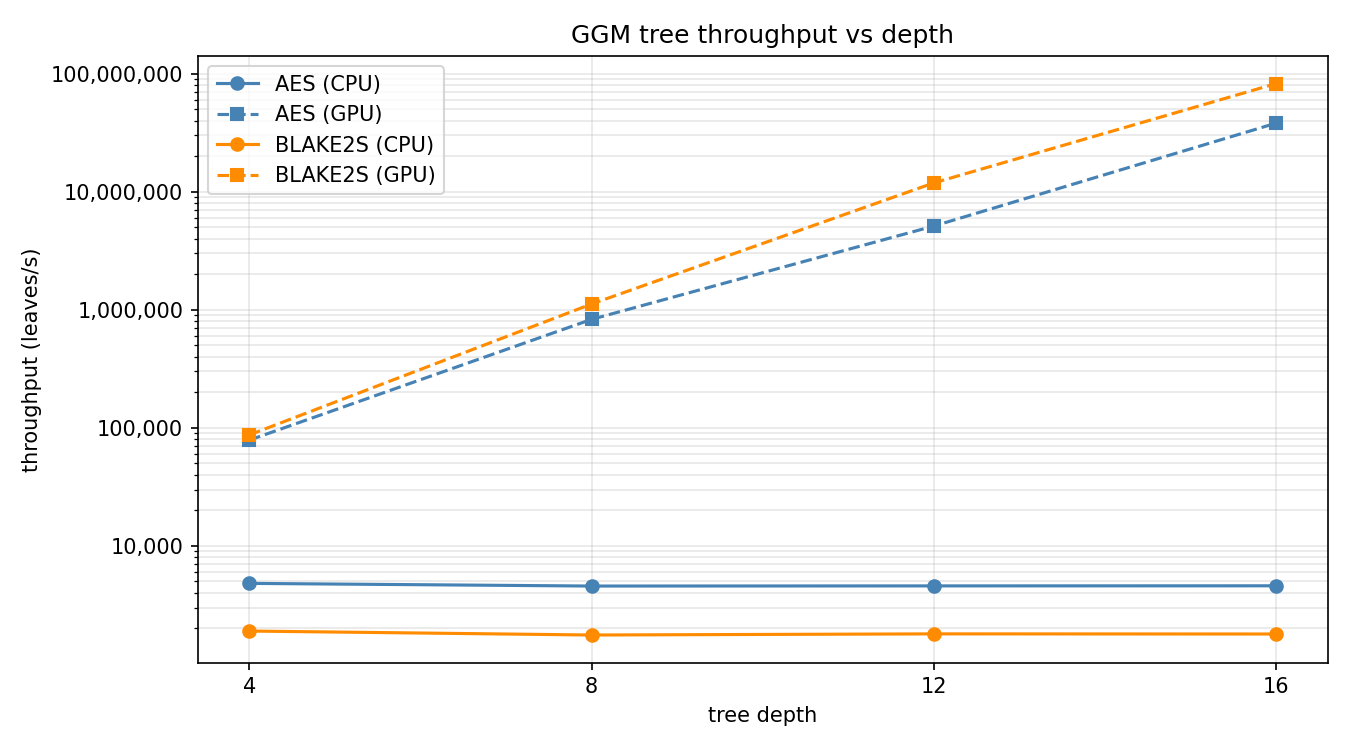
\includegraphics[width=\columnwidth]{benchmark_throughput.png}
\caption{Throughput (leaves/s, log scale) versus tree depth for all four backends}
\label{fig:throughput}
\end{figure}

\subsection{Speedup}
\label{sec:speedup}

\begin{figure}[H]
\centering
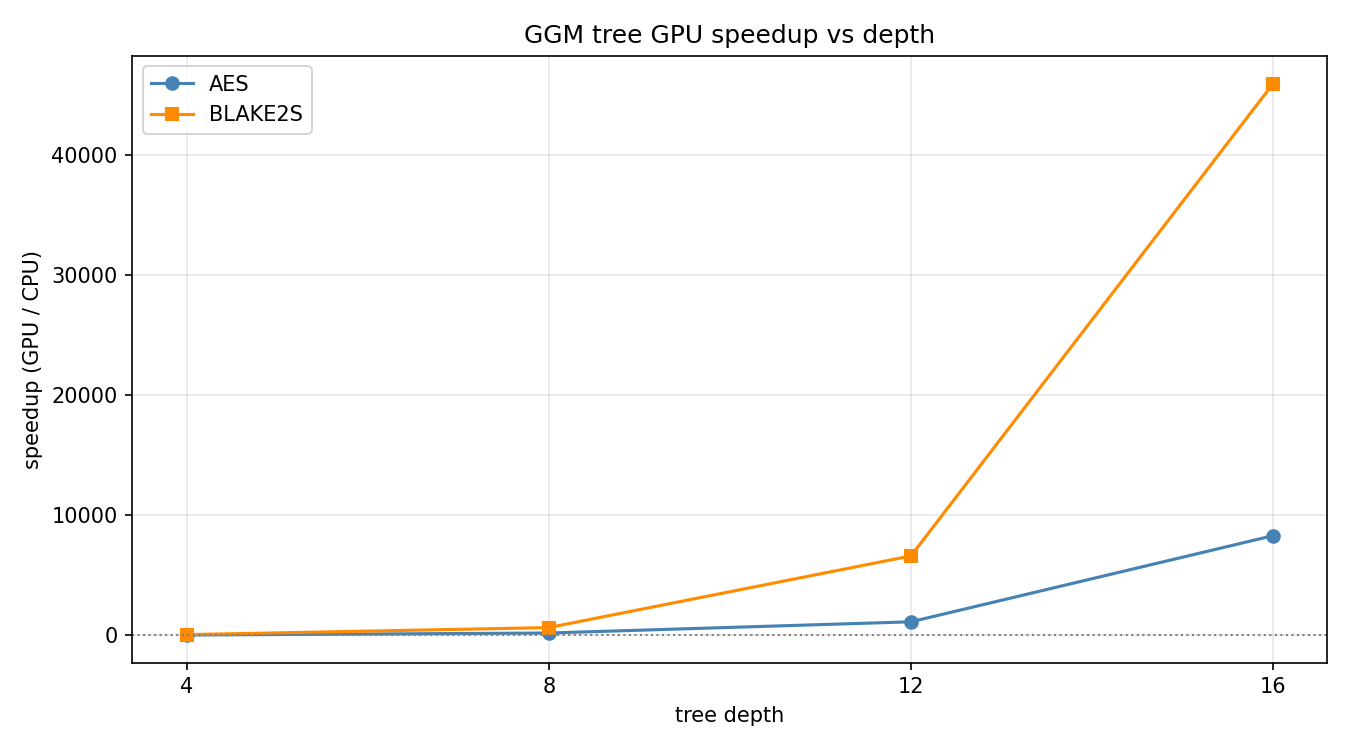
\includegraphics[width=\columnwidth]{benchmark_speedup.png}
\caption{GPU/CPU speedup versus tree depth}
\label{fig:speedup}
\end{figure}

Fig.~\ref{fig:speedup} shows GPU/CPU speedup as a function of depth. AES speedup grows from 16.3$\times$ at depth 4 to 8,298$\times$ at depth 16, while BLAKE2s grows from 45.8$\times$ to 45,975$\times$ over the same range. Both curves rise steeply with depth because the GPU time stays in the sub-millisecond range while the pure-Python CPU time grows linearly with the number of leaves. Unlike a comparison against an optimized library baseline, both speedups here are measured against from-scratch pure-Python implementations, so the ratios reflect the same kind of baseline for both PRGs and are directly comparable to one another.

\subsection{Performance \& Security Analysis}
\label{sec:tradeoff}

\paragraph{BLAKE2s Performance Benefits}
With both CPU baselines implemented from scratch, the comparison is on a fair footing, and BLAKE2s is the stronger one in every measured sense. It achieves the highest absolute GPU throughput (82.4 vs.\ 38.1 million leaves/s), and because its CPU baseline is also the slowest, it shows the largest GPU/CPU speedup (45,975$\times$ vs.\ 8,298$\times$). The same implementation discipline is applied to both PRGs, so the throughput and speedup differences are attributable to the primitives themselves rather than to uneven baselines.

\paragraph{Why BLAKE2s is faster on the GPU}
The performance gap aligns with the structure of the two primitives. BLAKE2s is built from add-rotate-xor operations on 32-bit words, which map directly onto GPU integer registers and arithmetic units with no table lookups. AES instead relies on S-box substitutions and finite-field arithmetic, where even with the S-box in constant memory, the per-thread key schedule and round structure involve more dependent operations and memory references. On hardware without dedicated AES instructions, the ARX design is simply a better fit for the GPU's execution model.

\paragraph{Security Tradeoffs}
Speed is only half of the tradeoff. AES-128 is the most studied block cipher in existence, and as a pseudorandom permutation, it provides a conservative and well-understood security foundation for the GGM PRG. BLAKE2s, while also well analyzed and designed with a notable security margin, is a hash-based construction where its keyed mode serves directly as a PRF. For applications that must expand very large GGM trees, our results suggest BLAKE2s offers materially higher throughput at a comparable security level, whereas AES may be preferred when its specific pedigree as a block cipher, or the availability of hardware AES instructions on the target platform, is decisive.

\paragraph{Scaling with tree size}
A final practical observation concerns how the GPU advantage grows with tree size. At depth 4, with only 16 leaves, both PRGs already show a GPU speedup (16.3$\times$ for AES, 45.8$\times$ for BLAKE2s), but the GPU is far from saturated, and the advantage is modest. As depth increases, each level exposes exponentially more independent nodes as the device fills, and the per leaf cost on the GPU falls by orders of magnitude while the CPU cost per leaf stays fixed. By depth 16, the GPU processes the full 65,536 leaf tree in under two milliseconds. This confirms that the GGM tree is an excellent match for GPU acceleration precisely because its parallelism grows with the problem size.

\subsection{Discussion}
The CPU paths are flat in throughput and separated only by the intrinsic per-call cost of the two primitives in Python. With BLAKE2s slower than AES, the GPU paths scale with available parallelism and favor BLAKE2s by more than 2$\times$ in absolute throughput. Because both CPU baselines share the same implementation approach, the speedup ratios are directly comparable. The defensible conclusion is that for large-scale GGM expansion on commodity GPUs without AES hardware support, BLAKE2s is the stronger default, reserving AES for cases where its block cipher semantics or hardware support are specifically required.

\section{Conclusion}
We implemented the GGM PRF tree construction from scratch on both CPU and GPU using two length-doubling PRGs, AES-128 and BLAKE2s, and verified the GPU kernels to be byte exact against validated CPU references for both primitives. On a CUDA GPU, the implementation reaches 82.4 million leaves/s for BLAKE2s and 38.1 million for AES at depth 16, with speedups up to 45,975$\times$ and 8,298$\times$ respectively over Python baselines. Because both CPU baselines were written from scratch, the comparison is fair, and BLAKE2s emerges as the stronger primitive on both throughput and speedup. This is consistent with its ARX design, fitting the GPU execution model better than AES's table-driven rounds. We also showed that the GPU advantage grows with tree size, which is as expected from the construction's level parallelism. Future work could include a CUDA implementation without the CuPy layer for the bonus objective, an AES-NI or optimized C CPU baseline to quantify the cost of approaches, and extending the comparison to additional PRGs.

\section*{Code Availability}
The complete CPU and GPU implementation, correctness suite, and benchmark harness are available at \url{https://github.com/ryluo-04/ece268-ggm-tree}.

\begin{thebibliography}{00}
\bibitem{ggm1986} O. Goldreich, S. Goldwasser, and S. Micali, ``How to construct random functions,'' \textit{Journal of the ACM}, vol. 33, no. 4, pp. 792--807, 1986.
\bibitem{fips197} National Institute of Standards and Technology, ``Advanced Encryption Standard (AES),'' FIPS PUB 197, 2001.
\bibitem{rfc7693} M.-J. Saarinen and J.-P. Aumasson, ``The BLAKE2 Cryptographic Hash and Message Authentication Code (MAC),'' RFC 7693, 2015.
\end{thebibliography}

\end{document}